\subsubsection{UC4 - Visualizza grafico}
\begin{figure}[h]
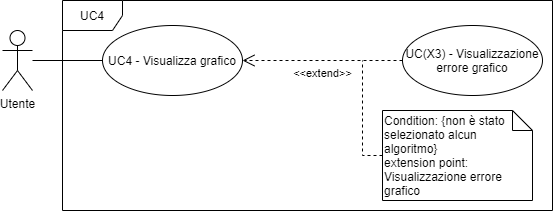
\includegraphics[width=\linewidth]{section/Images/UC4VisualizzaGrafico.png}
\centering
\caption{UC4 - Visualizza grafico}
\end{figure}
\begin{itemize}
	\item \textbf{Attore primario}: Utente.
	\item \textbf{Precondizioni}: L'utente ha caricato un file contenente dei dati [UC1] e ha scelto un algoritmo da visualizzare [UCX].
	\item \textbf{Postcondizioni}: Viene visualizzato il grafico richiesto.
	\item \textbf{Scenario principale}:
		\begin{enumerate}
			\item L'utente seleziona la funzionalità "visualizza grafico";
		\end{enumerate}
	\item \textbf{Estensioni}:
	\begin{enumerate}[(a)]
		\item Nel caso in cui non è stato selezionato alcun algoritmo:
		\begin{enumerate}[1.]
			\item il grafico non viene visualizzato;
			\item viene visualizzato un errore esplicativo [UCX3].
		\end{enumerate}
	\end{enumerate}
\end{itemize}